\chapter{Introduction}

This chapter is dedicated to the general introduction of the problem at hand and previous work and research that is relevant for this project.

\gls{ml} and Neural Networks have shown to be extremely potent and versatile in solving vast variety of problems across different fields. One research field that has been popular and challenging in the last few years is \gls{co}. \gls{co} includes problems such as \gls{mis} and \gls{mwm}. Such problems can be viewed in the context of graphs. \gls{gnn} is a subclass of Neural Networks designed specifically for solving problems related to graphs, but there are many problems that have not yet been solved efficiently with \gls{gnn}s. This work attemps to find out whether a \gls{gnn} can be worth using for solving \gls{mwm} 

\section{Background}

Many researches have been done related to \gls{gnn}s in the past years and some of them have shown mixed results. Lorenzo Brusca and Lars C. P. M. Quaedvlieg et al. \cite{brusca2023maximum} showed a self-training \gls{gnn} for \gls{mis}

\section{Project structure}

The rest of this document has the following structure:

\begin{enumerate}
\item Approach
\item Training
\item Results
\item Conclusion
\end{enumerate}


\subsection{Listings}
You can do listings, like in Listing~\ref{ListingReference}
\begin{lstlisting}[caption={[Short caption]Look at this cool listing. Find the rest in Appendix~\ref{Listing}},label=ListingReference]
$ java -jar myAwesomeCode.jar
\end{lstlisting}

You can also do language highlighting for instance with Golang:
And in line~\ref{LineThatDoesSomething} of Listing~\ref{ListingGolang} you can see that we can ref to lines in listings.

\begin{lstlisting}[caption={Hello world in Golang},label=ListingGolang,escapechar=|]
package main

import "fmt"

func main() {
    fmt.Println("hello world") |\label{LineThatDoesSomething}|
}

\end{lstlisting}

\subsection{Figures}

Example of a centred figure
\begin{figure}[H]
    \centering
    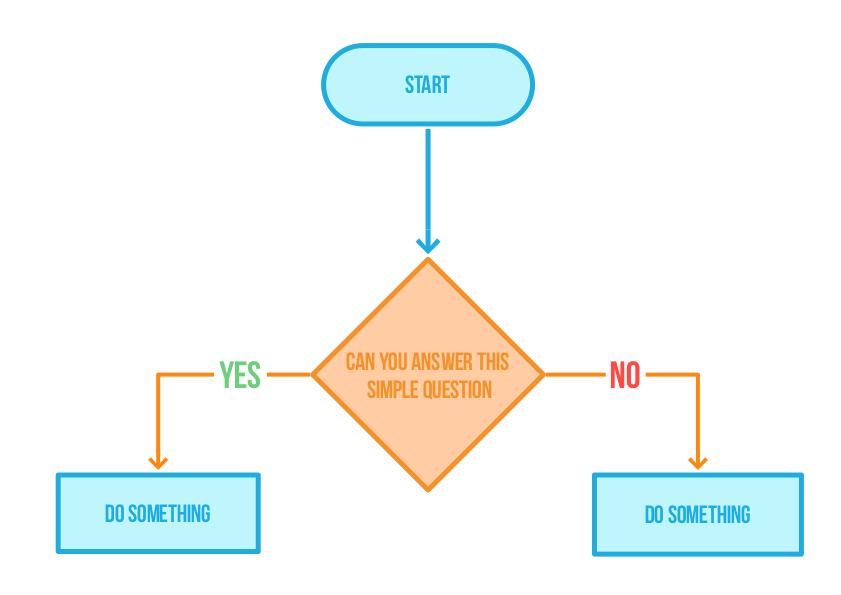
\includegraphics[scale=0.5]{figures/Flowchart}
    \caption{Caption for flowchart}
  	\medskip 
	\hspace*{15pt}\hbox{\scriptsize Credit: Acme company makes everything \url{https://acme.com/}}
    \label{FlowchartFigure}
\end{figure}

\subsection{Tables}

We can also do tables. Protip: use \url{https://www.tablesgenerator.com/} for generating tables.
\begin{table}[H]
\centering
\caption{Caption of table}
\label{TableLabel}
\begin{tabular}{|l|l|l|}
\hline
Title1 & Title2 & Title3 \\ \hline
data1  & data2  & data3  \\ \hline
\end{tabular}
\end{table}

\subsection{\gls{git}}

\gls{git} is fun, use it!